\chapter{Рисунки, поясняющие работу некоторых функций}
%\label{cha:appendix1}

%\begin{figure}
%\centering
%\caption{Картинка в приложении. Страшная и ужасная.}
%\end{figure}
\begin{figure}[h!]
	\centering
	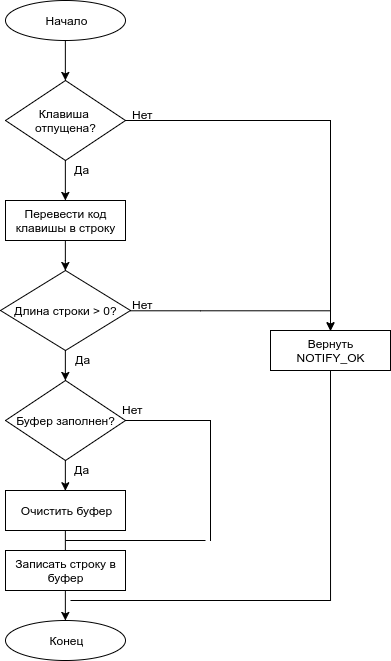
\includegraphics[width=0.6\textwidth]{img/diagram3.png}
	\caption{Алгоритм работы init-функции}
	\label{fig:spire02}
\end{figure}
\begin{figure}[h!]
	\centering
	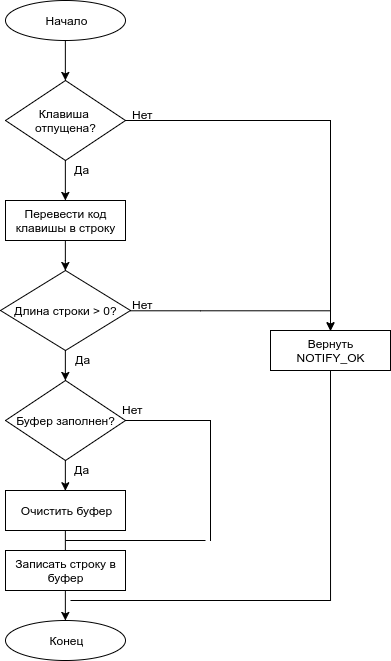
\includegraphics[width=0.6\textwidth]{img/diagram3.png}
	\caption{Алгоритм работы функции-обработчика}
	\label{fig:spire03}
\end{figure}
%%% Local Variables: 
%%% mode: latex
%%% TeX-master: "rpz"
%%% End: 
